\documentclass[10pt,adobefonts,fancyhdr,hyperref,UTF8]{ctexbook}

\usepackage{multirow}
% for \soul 删除线
\usepackage{ulem}
% 表头斜线
\usepackage{diagbox}

\makeatletter
\usepackage[centering,paperwidth=180mm,paperheight=230mm,%
body={390pt,530pt},marginparsep=10pt,marginpar=50pt]{geometry}
\usepackage{color}
\usepackage{enumitem}
\usepackage{fancyvrb}
\usepackage[bottom,perpage,symbol*]{footmisc}
\usepackage{graphicx}
\usepackage[hidelinks]{hyperref}
\usepackage{makeidx}
\usepackage[toc]{multitoc}
\usepackage{pifont}
\usepackage{underscore}
\usepackage{amsmath}

\DefineFNsymbols*{chinese}{{\ding{172}}{\ding{173}}{\ding{174}}{\ding{175}}%
{\ding{176}}{\ding{177}}{\ding{178}}{\ding{179}}{\ding{180}}{\ding{181}}}
\setfnsymbol{chinese}

\hypersetup{bookmarksnumbered=true,bookmarksdepth=2}

\CTEXsetup[number={\thechapter}]{chapter}
\CTEXsetup[format+={\raggedleft}]{chapter}
\CTEXsetup[beforeskip={10pt}]{chapter}
\CTEXsetup[afterskip={30pt}]{chapter}
\def\CTEX@chapter@aftername{\par} % \CTEXsetup[aftername={\par}]{chapter}
\CTEXsetup[format+={\raggedright}]{section}
\CTEXsetup[beforeskip={-3.0ex plus -1ex minus -.2ex}]{section}
\CTEXsetup[afterskip={2.3ex plus .2ex minus 0.2ex}]{section}

\renewcommand \thefigure{\thechapter-\arabic{figure}}
\renewcommand \thetable{\thechapter-\arabic{table}}

\newcommand\figcaption[1]{\def\@captype{figure}\caption{#1}}
\newcommand\tabcaption[1]{\def\@captype{table}\caption{#1}}

\long\def\@caption#1[#2]#3{%
  \addcontentsline{\csname ext@#1\endcsname}{#1}%
    {\protect\numberline{\csname fnum@#1\endcsname}{ \ignorespaces #2}}% change "the" to "fnum@"
    \normalsize
    \@makecaption{\csname fnum@#1\endcsname}{\ignorespaces #3}}

\long\def\@makecaption#1#2{%
  \vskip\abovecaptionskip
  \sbox\@tempboxa{#1\quad#2}%
  \ifdim \wd\@tempboxa >\hsize
    #1\quad#2\par
  \else
    \global \@minipagefalse
    \hb@xt@\hsize{\hfil\box\@tempboxa\hfil}%
  \fi
  \vskip\belowcaptionskip}

\setlength\abovecaptionskip{0pt}
  
\setmainfont{Times New Roman}
%\setmainfont{Linux Libertine}
%\setmainfont{TeX Gyre Pagella}
\newfontfamily\urlfont{PT Sans Narrow}
%\setmonofont[AutoFakeBold=1.6,AutoFakeSlant=0.17,Mapping=tex-text-tt]{Inconsolata}
\setCJKfamilyfont{zhyou}{YouYuan}

\newcommand{\fn}[1]{\texttt{#1}}
\newcommand{\sfn}[1]{\texttt{\small #1}}
\newcommand{\kw}[1]{\textsf{#1}}
\newcommand{\myurl}[1]{{\urlfont #1}}
\newcommand{\mpar}[1]{\marginpar[\hfill\kaishu #1]{\kaishu #1}}
\newcommand{\mn}[1]{\texttt{\bs #1}}
\renewcommand{\today}{\the\year-\the\month-\the\day}
\newcommand\bs{\textbackslash}
\newcommand{\code}[1]{\small{\fontspec{Latin Modern Mono} #1}}

\newcommand\begindot{\begin{itemize}
[itemsep=2pt plus 2pt minus 2pt,%
topsep=3pt plus 2pt minus 2pt,%
parsep=0pt plus 2pt minus 2pt]}
\newcommand\myenddot{\end{itemize}}

\newcommand\beginnum{\begin{enumerate}
[itemsep=2pt plus 2pt minus 2pt,%
topsep=3pt plus 2pt minus 2pt,%
parsep=0pt plus 2pt minus 2pt]}
\newcommand\myendnum{\end{enumerate}}

\DefineVerbatimEnvironment%
  {Code}{Verbatim}
  {fontsize=\small,baselinestretch=0.9,xleftmargin=3mm}

\raggedbottom
%\setlength{\parskip}{1ex plus .5ex minus .5ex}

\def\FV@SetLineWidth{%
  \if@FV@ResetMargins\else
    \advance\leftmargin\@totalleftmargin
  \fi
  \advance\leftmargin\FV@XLeftMargin\relax
  \advance\rightmargin\FV@XRightMargin\relax
  \linewidth\hsize
  %\advance\linewidth-\leftmargin
  %\advance\linewidth-\rightmargin
  \hfuzz\FancyVerbHFuzz\relax}


\def\FV@SingleFrameLine#1{%
%% DG/SR modification end
  \hbox to\z@{%
    %\kern\leftmargin
%% DG/SR modification begin - Jun. 22, 1998
    \ifnum#1=\z@
      \let\FV@Label\FV@LabelBegin
    \else
      \let\FV@Label\FV@LabelEnd
    \fi
    \ifx\FV@Label\relax
%% DG/SR modification end
      \FancyVerbRuleColor{\vrule \@width\linewidth \@height\FV@FrameRule}%
%% DG/SR modification begin - Jun. 22, 1998
    \else
      \ifnum#1=\z@
        \setbox\z@\hbox{\strut\enspace\urlfont\FV@LabelBegin\strut}%
      \else
        \setbox\z@\hbox{\strut\enspace\urlfont\FV@LabelEnd\strut}%
      \fi
      \@tempdimb=\dp\z@
      \advance\@tempdimb -.5\ht\z@
      \@tempdimc=\linewidth
      \advance\@tempdimc -\wd\z@
      %\divide\@tempdimc\tw@
      \ifnum#1=\z@              % Top line
        \ifx\FV@LabelPositionTopLine\relax
          \FancyVerbRuleColor{\vrule \@width\linewidth \@height\FV@FrameRule}%
        \else
          \FV@FrameLineWithLabel
        \fi
      \else                     % Bottom line
        \ifx\FV@LabelPositionBottomLine\relax
          \FancyVerbRuleColor{\vrule \@width\linewidth \@height\FV@FrameRule}%
        \else
          \FV@FrameLineWithLabel
        \fi
      \fi
    \fi
%% DG/SR modification end
    \hss}}


%% DG/SR modification begin - May. 19, 1998
\def\FV@FrameLineWithLabel{%
  \ht\z@\@tempdimb\dp\z@\@tempdimb%
  \FancyVerbRuleColor{%
    \raise 0.5ex\hbox{\vrule \@width\@tempdimc \@height\FV@FrameRule}%
    \raise\@tempdimb\box\z@}}
%% DG/SR modification end


\def\FV@EndListFrame@Lines{%
  \begingroup
    %\vskip 0.5ex
    \baselineskip\z@skip
    \kern\FV@FrameSep\relax
%% DG/SR modification begin - May. 19, 1998
%%    \FV@SingleFrameLine
    \FV@SingleFrameLine{\@ne}%
%% DG/SR modification end
  \endgroup}

\newskip\mytopsep
\setlength{\mytopsep}{4pt plus 2pt minus 3pt}

\def\FV@ListVSpace{%
  \@topsepadd\mytopsep
  \if@noparlist\advance\@topsepadd\partopsep\fi
  \if@inlabel
    \vskip\parskip
  \else
    \if@nobreak
      \vskip\parskip
      \clubpenalty\@M
    \else
      \addpenalty\@beginparpenalty
      \@topsep\@topsepadd
      \advance\@topsep\parskip
      \addvspace\@topsep
    \fi
  \fi
  %\showthe \@topsepadd
  %\showthe \topsep
  %\showthe \partopsep
  %\showthe \parskip
  \global\@nobreakfalse
  \global\@inlabelfalse
  \global\@minipagefalse
  \global\@newlistfalse}

\def\FV@EndList{%
  \FV@ListProcessLastLine
  \FV@EndListFrame
  %\showthe \@topsepadd
  \@endparenv
  \endgroup
  \@endpetrue}

\def\theFancyVerbLine{\sffamily\scriptsize\arabic{FancyVerbLine}}

\DefineVerbatimEnvironment%
  {Codex}{Verbatim}
  {fontsize=\small,baselinestretch=0.9,xleftmargin=3mm,%
  frame=lines,labelposition=all,framesep=5pt}

\DefineVerbatimEnvironment%
  {Code}{Verbatim}
  {fontsize=\small,baselinestretch=0.9,xleftmargin=3mm}

\makeindex

\makeatother

\begin{document}
\sloppy
\newcommand\BookTitle{LeetCode题解}
\pagestyle{fancy}
\fancyhf{}
\fancyhead[RE]{\normalfont\small\rmfamily\nouppercase{\leftmark}}
\fancyhead[LO]{\normalfont\small\rmfamily\nouppercase{\rightmark}}
\fancyhead[LE,RO]{\thepage}
%\fancyfoot[LE,LO]{\small\normalfont\youyuan\BookTitle}

\makeatletter
\@openrightfalse
\makeatother

\frontmatter % 开始前言目录,页码用罗马数字

\include{title}

\tableofcontents

\mainmatter % 开始正文,页码用阿拉伯数字

\graphicspath{{images/}}

\chapter{Backtracking}

\section{Regular Expression Matching} %%%%%%%%%%%%%%%%%%%%%%

\subsubsection{Description}
Implement regular expression matching with support for \fn{'.'} and \fn{'*'}.

\fn{'.'} Matches any single character.
\fn{'*'} Matches zero or more of the preceding element.

The matching should cover the entire input string (not partial).

Some examples:
\begin{Code}
isMatch("aa","a") → false
isMatch("aa","aa") → true
isMatch("aaa","aa") → false
isMatch("aa", "a*") → true
isMatch("aa", ".*") → true
isMatch("ab", ".*") → true
isMatch("aab", "c*a*b") → true
\end{Code}

\subsubsection{Solution}

\begin{Code}
public boolean isMatch(String s, String p) {
    if (p.isEmpty()) {
        return s.isEmpty();
    } else if (p.length() == 1) {
        return s.length() == 1 && isEqual(s, p);
    } else if (p.charAt(1) != '*') {
        return s.length() > 0 && isEqual(s, p) && isMatch(s.substring(1), p.substring(1));
    } else {
        if (s.length() > 0 && isEqual(s, p)) {
            return isMatch(s, p.substring(2)) || isMatch(s.substring(1), p);
        } else {
            return isMatch(s, p.substring(2));
        }
    }
}

private boolean isEqual(String s, String p) {
    return s.charAt(0) == p.charAt(0) || p.charAt(0) == '.';
}
\end{Code}

\newpage

\section{Wildcard Matching} %%%%%%%%%%%%%%%%%%%%%%

\subsubsection{Description}
Implement wildcard pattern matching with support for \fn{'?'} and \fn{'*'}.

\fn{'?'} Matches any single character.
\fn{'*'} Matches any sequence of characters (including the empty sequence).

\begin{Code}
Some examples:
isMatch("aa","a") → false
isMatch("aa","aa") → true
isMatch("aaa","aa") → false
isMatch("aa", "*") → true
isMatch("aa", "a*") → true
isMatch("ab", "?*") → true
isMatch("aab", "c*a*b") → false
\end{Code}

\subsubsection{Solution}
\begin{Code}
public boolean isMatch2(String s, String p) {
    int is = 0, ip = 0, ks = -1, kp = -1;

    while (is < s.length()) {
        if (ip < p.length() && (s.charAt(is) == p.charAt(ip) || p.charAt(ip) == '?')) {
            is++;
            ip++;
        } else if (ip < p.length() && p.charAt(ip) == '*') {
            ks = is;
            kp = ip;
            ip++;
        } else if (kp != -1) {
            is = ++ks;
            ip = kp + 1;
        } else {
            return false;
        }
    }

    for ( ; ip < p.length() && p.charAt(ip) == '*'; ip++);
    return ip == p.length();
}
\end{Code}

\newpage

\section{Letter Combinations of a Phone Number} %%%%%%%%%%%%%%%%%%%%%%

\subsubsection{Description}
Given a digit string, return all possible letter combinations that the number could represent.

A mapping of digit to letters (just like on the telephone buttons) is given below.

\begin{center}
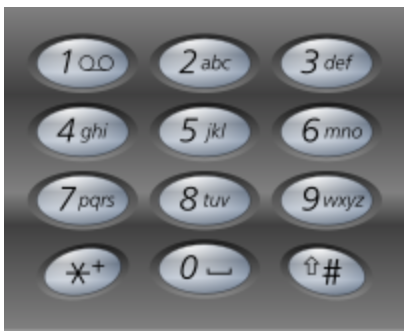
\includegraphics[width=150pt]{phone.png}\\
\figcaption{Phone Keyboard}\label{fig:phone-keyboard}
\end{center}

\textbf{Input:} Digit string \code{"23"}

\textbf{Output:} \code{["ad", "ae", "af", "bd", "be", "bf", "cd", "ce", "cf"]}.

\subsubsection{Solution I}

\begin{Code}
private final String[] ARR = {
        "", "", "abc", "def", "ghi", "jkl", "mno", "pqrs", "tuv", "wxyz"
};

public List<String> letterCombinations(String digits) {
    List<String> list = new LinkedList<>();
    if (!digits.isEmpty()) {
        helper(digits, 0, list, "");
    }
    return list;
}

private void helper(String digits, int start, List<String> list, String s) {
    if (start >= digits.length()) {
        list.add(s);
        return;
    }
    int n = digits.charAt(start) - '0';
    for (char c : ARR[n].toCharArray()) {
        helper(digits, start + 1, list, s + c);
    }
}
\end{Code}

\subsubsection{Solution II}

\begin{Code}

public List<String> letterCombinations(String digits) {
    LinkedList<String> queue = new LinkedList<String>();
    if (digits.length() == 0) {
        return queue;
    }

    Queue<String> next = new LinkedList<>();
    queue.add("");

    for (int i = 0; i < digits.length() && !queue.isEmpty(); ) {
        String s = queue.poll();
        int n = digits.charAt(i) - '0';
        for (char c : ARR[n].toCharArray()) {
            next.add(s + c);
        }
        if (queue.isEmpty()) {
            queue.addAll(next);
            next.clear();
            i++;
        }
    }
    return queue;
}
\end{Code}

\newpage

\section{Generate Parentheses} %%%%%%%%%%%%%%%%%%%%%%

\subsubsection{Description}
Given n pairs of parentheses, write a function to generate all combinations of well-formed parentheses.

For example, given \code{n = 3}, a solution set is:
\begin{Code}
[
  "((()))",
  "(()())",
  "(())()",
  "()(())",
  "()()()"
]
\end{Code}

\subsubsection{Solution}

\begin{Code}
public List<String> generateParenthesis(int n) {
    List<String> result = new LinkedList<String>();
    dfs(result, n, "", 0, 0);
    return result;
}

private void dfs(List<String> result, int n, String str, int left, int right) {
    if (left == n && right == n) {
        result.add(str);
        return;
    }
    if (left > n || right > n || left < right) {
        return;
    }
    dfs(result, n, str + "(", left + 1, right);
    dfs(result, n, str + ")", left, right + 1);
}
\end{Code}

\newpage

\section{Permutations} %%%%%%%%%%%%%%%%%%%%%%

\subsubsection{Description}
Given a collection of distinct numbers, return all possible permutations.

For example, \code{[1,2,3]} have the following permutations:
\begin{Code}
[
  [1,2,3],
  [1,3,2],
  [2,1,3],
  [2,3,1],
  [3,1,2],
  [3,2,1]
]
\end{Code}

\subsubsection{Solution}
\begin{Code}
public List<List<Integer>> permute(int[] nums) {
    List<List<Integer>> result = new ArrayList<List<Integer>>();
    permute(nums, result, 0);
    return result;
}

public void permute(int[] nums, List<List<Integer>> result, int start) {
    if (start >= nums.length) {
        List<Integer> list = new ArrayList<Integer>();
        for (Integer n : nums) {
            list.add(n);
        }
        result.add(list);
    }

    for (int i = start; i < nums.length; i++) {
        swap(nums, start, i);
        permute(nums, result, start + 1);
        swap(nums, start, i);
    }
}

public static void swap(int[] nums, int left, int right) {
    int temp = nums[left];
    nums[left] = nums[right];
    nums[right] = temp;
}
\end{Code}

\newpage

\section{Word Search} %%%%%%%%%%%%%%%%%%%%%%

\subsubsection{Description}
Given a 2D board and a word, find if the word exists in the grid.

The word can be constructed from letters of sequentially adjacent cell, where adjacent cells are those horizontally or vertically neighboring. The same letter cell may not be used more than once.

For example,
Given board =
\begin{Code}
[
  ['A','B','C','E'],
  ['S','F','C','S'],
  ['A','D','E','E']
]
\end{Code}

word = \code{"ABCCED"}, -> returns true,

word = \code{"SEE"}, -> returns true,

word = \code{"ABCB"}, -> returns false.

\subsubsection{Solution}

\begin{Code}
public boolean exist(char[][] board, String word) {
    for (int i = 0; i < board.length; i++) {
        for (int j = 0; j < board[0].length; j++) {
            if (dfs(board, i, j, word, 0)) {
                return true;
            }
        }
    }
    return false;
}

private boolean dfs(char[][] board, int i, int j, String word, int start) {
    if (start == word.length()) {
        return true;
    }
    if (i < 0 || i >= board.length || j < 0 || j >= board[0].length) {
        return false;
    }
    if (board[i][j] != word.charAt(start)) {
        return false;
    }

    board[i][j] ^= '#';
    boolean flag = dfs(board, i + 1, j, word, start + 1)
            || dfs(board, i - 1, j, word, start + 1)
            || dfs(board, i, j + 1, word, start + 1)
            || dfs(board, i, j - 1, word, start + 1);
    board[i][j] ^= '#';
    return flag;
}
\end{Code}

\newpage

\section{Word Search II} %%%%%%%%%%%%%%%%%%%%%%

\subsubsection{Description}
Given a 2D board and a list of words from the dictionary, find all words in the board.

Each word must be constructed from letters of sequentially adjacent cell, where adjacent cells are those horizontally or vertically neighboring. The same letter cell may not be used more than once in a word.

For example,
Given words = \code{["oath","pea","eat","rain"]} and board =
\begin{Code}
[
  ['o','a','a','n'],
  ['e','t','a','e'],
  ['i','h','k','r'],
  ['i','f','l','v']
]
\end{Code}
Return \code{["eat","oath"]}.

Note:
You may assume that all inputs are consist of lowercase letters a-z.

You would need to optimize your backtracking to pass the larger test. Could you stop backtracking earlier?

If the current candidate does not exist in all words' prefix, you could stop backtracking immediately. What kind of data structure could answer such query efficiently? Does a hash table work? Why or why not? How about a Trie? If you would like to learn how to implement a basic trie, please work on this problem: Implement Trie (Prefix Tree) first.

\subsubsection{Solution}

\begin{Code}
private class Trie {
    Trie[] nodes = new Trie[26];
    String word;
}

private void buildTrie(Trie trie, String word) {
    for (int i = 0; i < word.length(); i++) {
        if (trie.nodes[word.charAt(i) - 'a'] == null) {
            trie.nodes[word.charAt(i) - 'a'] = new Trie();
        }
        trie = trie.nodes[word.charAt(i) - 'a'];
    }
    trie.word = word;
}
\end{Code}

\newpage

\begin{Code}

public List<String> findWords(char[][] board, String[] words) {
    Trie trie = new Trie();
    for (String word : words) {
        buildTrie(trie, word);
    }
    Set<String> set = new HashSet<String>();
    for (int i = 0; i < board.length; i++) {
        for (int j = 0; j < board[0].length; j++) {
            dfs(set, board, i, j, trie);
        }
    }
    return new LinkedList<String>(set);
}

private void dfs(Set<String> set, char[][] board, int i, int j, Trie trie) {
    if (i < 0 || i >= board.length || j < 0 || j >= board[0].length) {
        return;
    }
    if (trie == null) {
        return;
    }
    char c = board[i][j];
    if (c < 'a' || c > 'z') {
        return;
    }
    trie = trie.nodes[c - 'a'];
    if (trie == null) {
        return;
    }
    if (trie.word != null) {
        set.add(trie.word);
    }

    board[i][j] ^= '#';
    dfs(set, board, i + 1, j, trie);
    dfs(set, board, i - 1, j, trie);
    dfs(set, board, i, j + 1, trie);
    dfs(set, board, i, j - 1, trie);
    board[i][j] ^= '#';
}
\end{Code}

\newpage

\section{Word Break} %%%%%%%%%%%%%%%%%%%%%%

\subsubsection{Description}
Given a non-empty string s and a dictionary wordDict containing a list of non-empty words, determine if s can be segmented into a space-separated sequence of one or more dictionary words. You may assume the dictionary does not contain duplicate words.

For example, given
s = \code{"leetcode"},
dict = \code{["leet", "code"]}.

Return true because \code{"leetcode"} can be segmented as \code{"leet code"}.

\subsubsection{Solution}

\begin{Code}
public boolean wordBreak(String s, List<String> wordDict) {
    int n = s.length();

    boolean[] dp = new boolean[n + 1];
    dp[0] = true;

    for (int i = 1; i <= s.length(); i++) {
        for (String word : wordDict) {
            int j = i - word.length();
            if (j >= 0 && dp[j] && s.substring(j, i).equals(word)) {
                dp[i] = true;
                break;
            }
        }
    }

    return dp[n];
}
\end{Code}

\newpage

\section{Word Break II} %%%%%%%%%%%%%%%%%%%%%%

\subsubsection{Description}
Given a non-empty string s and a dictionary wordDict containing a list of non-empty words, add spaces in s to construct a sentence where each word is a valid dictionary word. You may assume the dictionary does not contain duplicate words.

Return all such possible sentences.

For example, given
s = \code{"catsanddog"},
dict = \code{["cat", "cats", "and", "sand", "dog"]}.

A solution is \code{["cats and dog", "cat sand dog"]}.

\subsubsection{Solution}

\begin{Code}
public List<String> wordBreak(String s, List<String> wordDict) {
    HashMap<String, List<String>> cache = new HashMap<>();
    cache.put("", Arrays.asList(""));
    return dfs(s, new HashSet<String>(wordDict), cache);
}

private List<String> dfs(String s, HashSet<String> wordDict, HashMap<String, List<String>> cache) {
    if (cache.containsKey(s)) {
        return cache.get(s);
    }
    List<String> result = new LinkedList<>();
    for (int i = 0; i < s.length(); i++) {
        String t = s.substring(i);
        if (wordDict.contains(t)) {
            List<String> list = dfs(s.substring(0, i), wordDict, cache);
            if (list != null) {
                for (String ss : list) {
                    result.add((ss.length() > 0 ? ss + " " : "") + t);
                }
            }
        }
    }
    cache.put(s, result);
    return result;
}
\end{Code}

\newpage

\section{Combination Sum} %%%%%%%%%%%%%%%%%%%%%%

\subsubsection{Description}

Given a set of candidate numbers (C) (without duplicates) and a target number (T), find all unique combinations in C where the candidate numbers sums to T.

The same repeated number may be chosen from C unlimited number of times.

Note:

All numbers (including target) will be positive integers.

The solution set must not contain duplicate combinations.

For example, given candidate set \code{[2, 3, 6, 7]} and target 7,

A solution set is:
\begin{code}
[
  [7],
  [2, 2, 3]
]
\end{code}

\subsubsection{Solution I}

\begin{Code}
public List<List<Integer>> combinationSum(int[] candidates, int target) {
    List<List<Integer>> result = new LinkedList<>();
    helper(candidates, result, new LinkedList<>(), target, 0);
    return result;
}

private void helper(int[] candidates, List<List<Integer>> result, List<Integer> list, int target, int index) {
    if (target < 0) {
        return;
    } else if (target == 0) {
        result.add(new LinkedList<>(list));
        return;
    } else if (index >= candidates.length) {
        return;
    }

    list.add(candidates[index]);
    helper(candidates, result, list, target - candidates[index], index);
    list.remove(list.size() - 1);

    helper(candidates, result, list, target, index + 1);
}

\end{Code}

\newpage

\subsubsection{Solution II}

\begin{Code}

public List<List<Integer>> combinationSum(int[] candidates, int target) {
    List<List<Integer>> result = new LinkedList<>();
    dfs(candidates, target, 0, result, new LinkedList<Integer>());
    return result;
}

private void dfs(int[] candidates, int target, int start, List<List<Integer>> result, List<Integer> list) {
    if (target < 0) {
        return;
    }
    if (target == 0) {
        result.add(new LinkedList<>(list));
        return;
    }
    for (int i = start; i < candidates.length; i++) {
        list.add(candidates[i]);
        dfs(candidates, target - candidates[i], i, result, list);
        list.remove(list.size() - 1);
    }
}
\end{Code}

\newpage

\section{Combination Sum II} %%%%%%%%%%%%%%%%%%%%%%

\subsubsection{Description}
Given a collection of candidate numbers (C) and a target number (T), find all unique combinations in C where the candidate numbers sums to T.

Each number in C may only be used once in the combination.

Note:

All numbers (including target) will be positive integers.

The solution set must not contain duplicate combinations.

For example, given candidate set \code{[10, 1, 2, 7, 6, 1, 5]} and target 8,

A solution set is:
\begin{Code}
[
  [1, 7],
  [1, 2, 5],
  [2, 6],
  [1, 1, 6]
]
\end{Code}

\subsubsection{Solution I}

\begin{Code}
public List<List<Integer>> combinationSum(int[] candidates, int target) {
    List<List<Integer>> result = new LinkedList<>();
    Arrays.sort(candidates);
    helper(candidates, result, new LinkedList<>(), target, 0);
    return result;
}

private void helper(int[] candidates, List<List<Integer>> result, List<Integer> list, int target, int index) {
    if (target < 0) {
        return;
    } else if (target == 0) {
        result.add(new LinkedList<>(list));
        return;
    } else if (index >= candidates.length) {
        return;
    }

    list.add(candidates[index]);
    helper(candidates, result, list, target - candidates[index], index + 1);
    list.remove(list.size() - 1);

    for ( ; index < candidates.length - 1 && candidates[index + 1] == candidates[index]; index++);

    helper(candidates, result, list, target, index + 1);
}
\end{Code}

\newpge

\subsubsection{Solution II}

\begin{Code}
public List<List<Integer>> combinationSum(int[] candidates, int target) {
    List<List<Integer>> result = new LinkedList<List<Integer>>();
    Arrays.sort(candidates);
    dfs(candidates, 0, target, result, new LinkedList<Integer>());
    return result;
}

private void dfs(int[] candidates, int start, int target, List<List<Integer>> result, List<Integer> path) {
    if (target < 0) {
        return;
    }

    if (target == 0) {
        result.add(new LinkedList<Integer>(path));
        return;
    }

    for (int i = start; i < candidates.length; i++) {
        if (i > start && candidates[i] == candidates[i - 1]) {
            continue;
        }

        path.add(candidates[i]);

        // 关键是这里变成i + 1
        dfs(candidates, i + 1, target - candidates[i], result, path);
        path.remove(path.size() - 1);
    }
}
\end{Code}

\newpage

\section{Combination Sum III} %%%%%%%%%%%%%%%%%%%%%%

\subsubsection{Description}
Find all possible combinations of k numbers that add up to a number n, given that only numbers from 1 to 9 can be used and each combination should be a unique set of numbers.

\textbf{Example 1:}

Input: \code{k = 3, n = 7}

Output: \code{[[1,2,4]]}

\textbf{Example 2:}

Input: \code{k = 3, n = 9}

Output: \code{[[1,2,6], [1,3,5], [2,3,4]]}

\subsubsection{Solution I}

\begin{Code}
public List<List<Integer>> combinationSum(int k, int n) {
    List<List<Integer>> result = new LinkedList<>();
    helper(k, n, result, new LinkedList<>(), 1);
    return result;
}

private void helper(int k, int n, List<List<Integer>> result, List<Integer> list, int cur) {
    if (n == 0 && k == 0) {
        result.add(new LinkedList<>(list));
        return;
    }

    if (cur > 9) {
        return;
    }

    list.add(cur);
    helper(k - 1, n - cur, result, list, cur + 1);
    list.remove(list.size() - 1);

    helper(k, n, result, list, cur + 1);
}
\end{Code}

\newpage

\subsubsection{Solution II}

\begin{Code}
public List<List<Integer>> combinationSum(int k, int n) {
    List<List<Integer>> result = new LinkedList<>();
    dfs(n, k, 1, result, new LinkedList<Integer>());
    return result;
}

private void dfs(int target, int k, int start, List<List<Integer>> result, List<Integer> list) {
    if (target == 0 && k == 0) {
        result.add(new LinkedList<>(list));
        return;
    }
    if (target <= 0 || k <= 0) {
        return;
    }
    for (int i = start; i <= 9; i++) {
        list.add(i);
        dfs(target - i, k - 1, i + 1, result, list);
        list.remove(list.size() - 1);
    }
}
\end{Code}

\newpage

\section{Combination Sum IV} %%%%%%%%%%%%%%%%%%%%%%

\subsubsection{Description}
Given an integer array with all positive numbers and no duplicates, find the number of possible combinations that add up to a positive integer target.

\textbf{Example:}

nums = \code{[1, 2, 3]}
target = 4

The possible combination ways are:
\begin{Code}
(1, 1, 1, 1)
(1, 1, 2)
(1, 2, 1)
(1, 3)
(2, 1, 1)
(2, 2)
(3, 1)
\end{Code}

Note that different sequences are counted as different combinations.

Therefore the output is 7.

\textbf{Follow up:}

What if negative numbers are allowed in the given array?

How does it change the problem?

What limitation we need to add to the question to allow negative numbers?

\subsubsection{Solution}

\begin{Code}
public int combinationSum4(int[] nums, int target) {
    int[] dp = new int[target + 1];
    // 这里排序便于之后break
    Arrays.sort(nums);
    // 这里0为什么是1呢,我开始也不解,
    // 其实就是说如果组合中带的刚好是当前数,那么组合数只有1种。
    // 比如target为3的时候,遍历到了nums中的3,那么只有1种可能。
    dp[0] = 1;
    for (int i = 1; i <= target; i++) {
        for (int num : nums) {
            if (num > i) {
                break;
            } else {
                dp[i] += dp[i - num];
            }
        }
    }
    return dp[target];
}
\end{Code}

\newpage

\section{N-Queens} %%%%%%%%%%%%%%%%%%%%%%

\subsubsection{Description}
The n-queens puzzle is the problem of placing n queens on an n×n chessboard such that no two queens attack each other.

\begin{center}
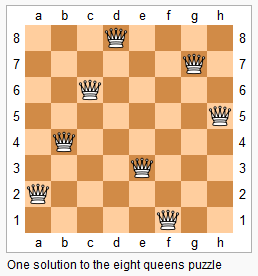
\includegraphics[width=100pt]{8-queens.png}\\
\end{center}

Given an integer n, return all distinct solutions to the n-queens puzzle.

Each solution contains a distinct board configuration of the n-queens' placement, where \code{'Q'} and \fn{'.'} both indicate a queen and an empty space respectively.

For example,

There exist two distinct solutions to the 4-queens puzzle:

\begin{Code}
[
 [".Q..",  // Solution 1
  "...Q",
  "Q...",
  "..Q."],

 ["..Q.",  // Solution 2
  "Q...",
  "...Q",
  ".Q.."]
]
\end{Code}

\newpage

\subsubsection{Solution}

\begin{Code}
public List<List<String>> solveNQueens(int n) {
    List<List<String>> result = new LinkedList<>();
    /**
     * 这里f[i]表示第i行皇后应该放置在第几列
     */
    int[] f = new int[n];
    dfs(f, result, 0);
    return result;
}

private void dfs(int[] f, List<List<String>> result, int row) {
    if (row == f.length) {
        List<String> list = new LinkedList<>();
        char[] c = new char[f.length];
        for (int i = 0; i < f.length; i++) {
            Arrays.fill(c, '.');
            for (int j = 0; j < f.length; j++) {
                if (j == f[i]) {
                    c[j] = 'Q';
                    break;
                }
            }
            list.add(String.valueOf(c));
        }
        result.add(list);
    }
    /**
     * 对于当前第row行,一列一列地尝试放置皇后,看是否合法,j表示列,如果合法则保存到f中
     */
    for (int j = 0; j < f.length; j++) {
        if (isValid(f, row, j)) {
            f[row] = j;
            dfs(f, result, row + 1);
        }
    }
}

private boolean isValid(int[] f, int row, int col) {
    for (int i = 0; i < row; i++) {
        if (f[i] == col) {
            return false;
        }
        if (Math.abs(i - row) == Math.abs(f[i] - col)) {
            return false;
        }
    }
    return true;
}
\end{Code}

\newpage

\section{N-Queens II} %%%%%%%%%%%%%%%%%%%%%%

\subsubsection{Description}

Follow up for N-Queens problem.

Now, instead outputting board configurations, return the total number of distinct solutions.

\subsubsection{Solution}

\begin{Code}
private int total;

public int totalNQueens(int n) {
    int[] f = new int[n];
    dfs(f, 0);
    return total;
}

private void dfs(int[] f, int row) {
    if (row == f.length) {
        total++;
        return;
    }
    for (int j = 0; j < f.length; j++) {
        if (isValid(f, row, j)) {
            f[row] = j;
            dfs(f, row + 1);
        }
    }
}

private boolean isValid(int[] f, int row, int col) {
    for (int i = 0; i < row; i++) {
        if (f[i] == col) {
            return false;
        }
        if (Math.abs(i - row) == Math.abs(f[i] - col)) {
            return false;
        }
    }
    return true;
}
\end{Code}

\newpage

\section{Subsets} %%%%%%%%%%%%%%%%%%%%%%

\subsubsection{Description}

Given a set of distinct integers, nums, return all possible subsets.

Note: The solution set must not contain duplicate subsets.

For example,
If nums = \code{[1,2,3]}, a solution is:

\begin{Code}
[
  [3],
  [1],
  [2],
  [1,2,3],
  [1,3],
  [2,3],
  [1,2],
  []
]
\end{Code}

\subsubsection{Solution I}

\begin{Code}
public List<List<Integer>> subsets(int[] nums) {
    List<List<Integer>> result = new LinkedList<List<Integer>>();

    if (nums.length == 0) {
        return result;
    }

    subsets(nums, 0, result, new LinkedList<Integer>());

    return result;
}

private void subsets(int[] nums, int start, List<List<Integer>> list, List<Integer> path) {
    if (start == nums.length) {
        list.add(new LinkedList<Integer>(path));
        return;
    }

    path.add(nums[start]);
    subsets(nums, start + 1, list, path);
    path.remove(path.size() - 1);

    subsets(nums, start + 1, list, path);
}
\end{Code}

\newpage

\subsubsection{Solution II}

\begin{Code}
public List<List<Integer>> subsets(int[] nums) {
    List<List<Integer>> result = new LinkedList<List<Integer>>();

    if (nums.length == 0) {
        return result;
    }

    Arrays.sort(nums);
    subsets(nums, 0, result, new LinkedList<Integer>());
    return result;
}

private void subsets(int[] nums, int start, List<List<Integer>> result, List<Integer> path) {
    result.add(new LinkedList<Integer>(path));
    for (int i = start; i < nums.length; i++) {
        path.add(nums[i]);
        subsets(nums, i + 1, result, path);
        path.remove(path.size() - 1);
    }
}
\end{Code}

\newpage

\section{Subsets II} %%%%%%%%%%%%%%%%%%%%%%

\subsubsection{Description}
Given a collection of integers that might contain duplicates, nums, return all possible subsets.

Note: The solution set must not contain duplicate subsets.

For example,
If nums = \code{[1,2,2]}, a solution is:

\begin{Code}
[
  [2],
  [1],
  [1,2,2],
  [2,2],
  [1,2],
  []
]
\end{Code}

\subsubsection{Solution}

\begin{Code}
public List<List<Integer>> subsetsWithDup(int[] nums) {
    List<List<Integer>> result = new LinkedList<List<Integer>>();

    if (nums.length == 0) {
        return result;
    }
    /**
     * 千万别掉了排序
     */
    Arrays.sort(nums);
    subsetsWithDup(nums, 0, result, new LinkedList<Integer>());

    return result;
}

private void subsetsWithDup(int[] nums, int start, List<List<Integer>> list, List<Integer> path) {
    if (start == nums.length) {
        list.add(new LinkedList<Integer>(path));
        return;
    }

    path.add(nums[start]);
    subsetsWithDup(nums, start + 1, list, path);
    path.remove(path.size() - 1);

    // 既然不带当前字符,那后面如果重复的都别带,否则就是带了当前字符的子集
    for ( ; start + 1 < nums.length && nums[start + 1] == nums[start]; start++);
    subsetsWithDup(nums, start + 1, list, path);
}
\end{Code}


\appendix % 开始附录,章用字母编号
\printindex

\end{document}
